\documentclass[fleqn, onecolumn]{article}
\usepackage{amsmath}
%\usepackage[landscape]{geometry}
\usepackage{graphicx}
\usepackage{subfig}
\usepackage{fullpage}
%\usepackage{hyperref}
%\usepackage{listings}
\setlength{\parindent}{0in}

\begin{document}
\title{LEDA Memo: 8 Bit Sampling of LWA Data}
%\date{}
\author{Terry Filiba}
\maketitle

\section{Summary}
In order to determine the suitability of an 8 bit ADC for sampling LWA data, we analyzed data taken every 15 minutes over a 24 hour period from 6 LWA dual pol stands. 
The data was captured using the currently available 12 bit ADCs. 
The following plots and statistics were produced using all of the captured data.
\\

\begin{figure}[h] 
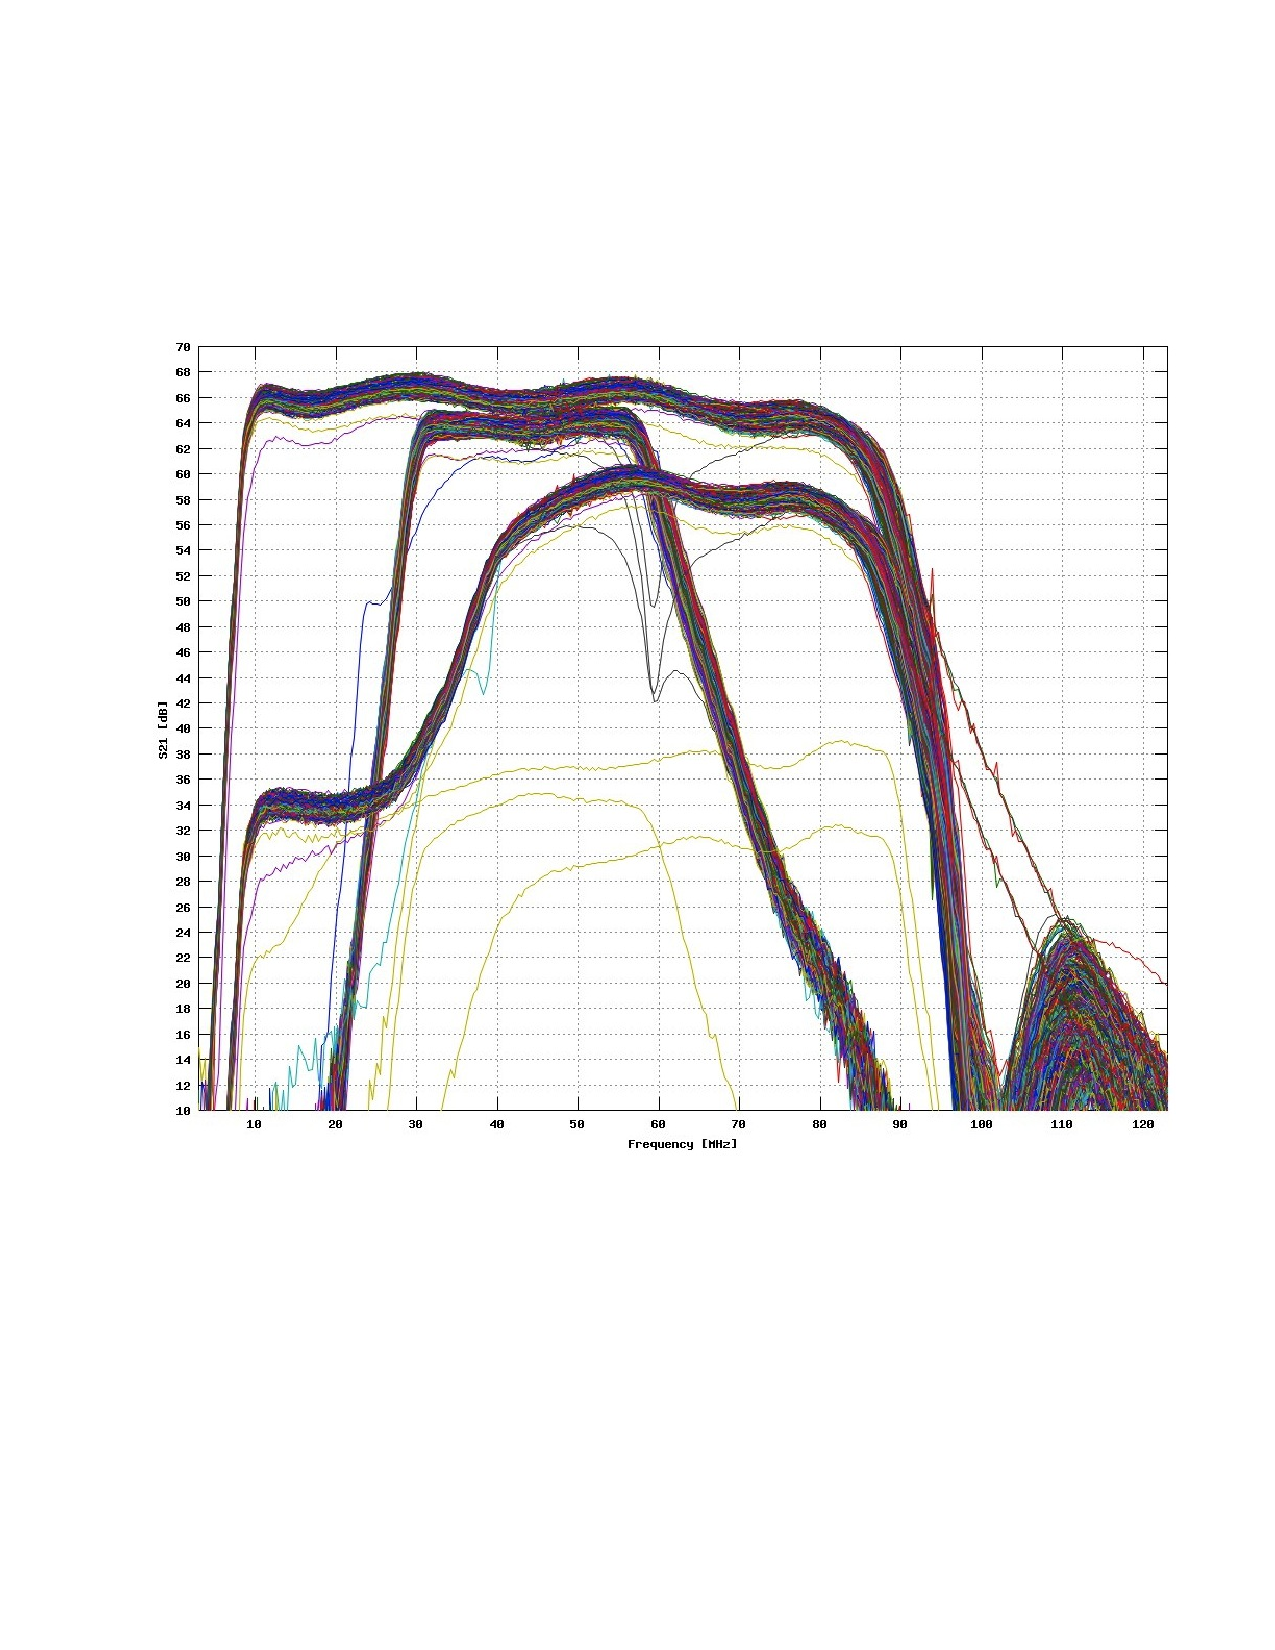
\includegraphics[width=0.9\textwidth]{filter_response.pdf}
\caption{ARX filter response. Refer to the memo ``Manufacturing Tests of the Analog Receiver (ARX) Boards" for more information on the filters.} 
\label{filterresponse}
\end{figure} 

Figure \ref{filterresponse} shows the  frequency responses of all the available LWA filters.
The "split bandwidth" filter set that was selected for this experiment has a
main passband from 40 to 90 MHz, and an attenuated passband
from 10 to 40 MHz (the staircase passband shown in figure \ref{filterresponse}).  
The filter was configured as follows: \\
Filter Config:  Split Bandwidth, ARX setting of ``0" \\
Split Bandwidth Attenuation:  24 dB (maximum), ARX setting of ``15"  \\
First Attenuator:  16 dB (out of 30 dB), AT1 = ``08" \\
Second Attenuator:  12 dB (out of 30 dB), AT2 = ``06" \\



Analysis of the data showed that at least 97\% of the samples lie within the range $[-128,128)$. 
Therefore, without adjusting any gains there would be $< 3\%$ error due to saturation using an 8 bit ADC.
If the ADC gain is set so that the RMS is $20$, the error rate of the ADC gets even lower. 
With the sampled data rescaled, saturation would only occur in $<0.001\%$ of the samples using an 8 bit ADC (an error rate of $10^{-5}$). 

Based on this analysis, we recommend using an 8 bit ADC to sample LEDA data from the LWA. If the gains are adjusted appropriately, there will be very little loss due to saturation.

\begin{table}[h]
$ \begin{array}{c||c|c|c}  
\text{Stand} & \text{RMS} & \text{samples }\in [-128,128) & \text{samples }\in [-128,128)\text{ with RMS}=20 \\ 
Stand001X & 34.118798 & 99.9896\% & 99.9998\% \\ 
Stand001Y & 28.544380 & 99.9988\% & 99.9999\% \\ 
Stand010X & 55.174325 & 98.0064\% & 99.9997\% \\ 
Stand010Y & 46.112851 & 99.4528\% & 99.9999\% \\ 
Stand054X & 43.717739 & 99.6627\% & 99.9996\% \\ 
Stand054Y & 47.889111 & 99.2436\% & 99.9999\% \\ 
Stand248X & 26.123759 & 99.9996\% & 99.9998\% \\ 
Stand248Y & 30.7075512 & 99.9988\% & 100.0000\% \\ 
Stand251X & 58.756399 & 97.0939\% & 99.9996\% \\ 
Stand251Y & 58.047033 & 97.2851\% & 99.9997\% \\ 
Stand258X & 27.404131 & 99.9993\% & 99.9998\% \\ 
Stand258Y & 28.3805394 & 99.9995\% & 100.0000\%
 \end{array}  
$
\end{table}

\section{Histograms}
The rest of the memo contains histograms of the data from each stand-pol. 
Each histogram is shown in linear and log scale, to highlight the peakedness and short tails of each distribution. 
The blue bars highlight the samples that could be represented with 8 bits without gain adjustment. 
The yellow bars show the samples that would not saturate if the gain was adjusted so that the RMS is $20$.
The log plots of the data emphasize the short tails in the histogram, showing that adjusting the gain will be an effective way to reduce the saturation rate. 

%\newpage

\begin{figure}[h] 				\subfloat{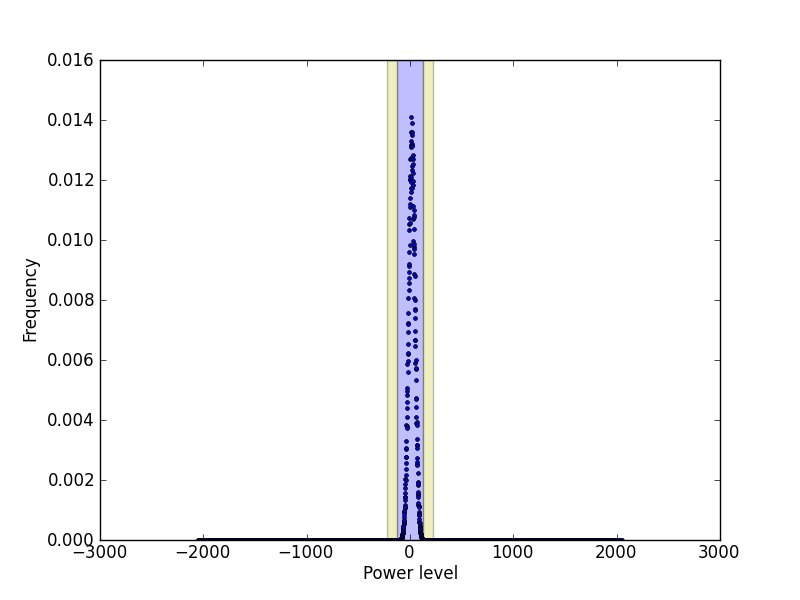
\includegraphics[width=0.5\textwidth]{plots/Stand001Xhist.png}} 				\subfloat{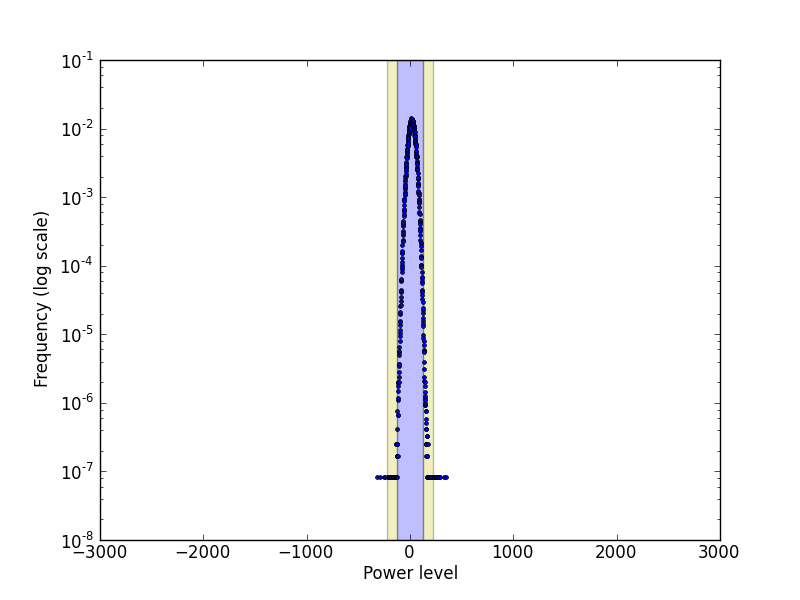
\includegraphics[width=0.5\textwidth]{plots/Stand001Xhist_log.png}} 				\caption{Data from Stand001X. RMS is 34.1188 Samples used : 3792000000. If the RMS is unchanged 99.9896 percent of the samples will lie within [-128,128).  				 With an RMS of 20, 99.9998 percent of the samples will lie within [-128,128).} 				\end{figure} 

\begin{figure}[h] 				\subfloat{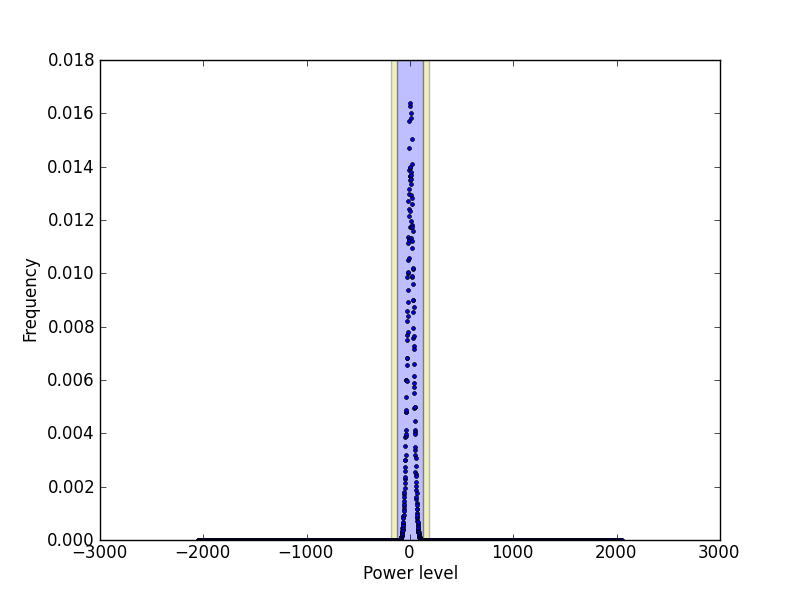
\includegraphics[width=0.5\textwidth]{plots/Stand001Yhist.png}} 				\subfloat{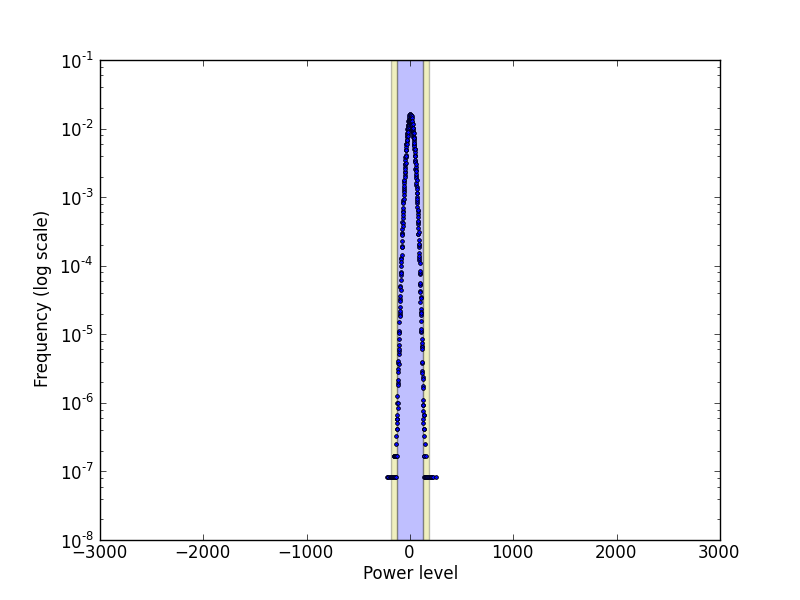
\includegraphics[width=0.5\textwidth]{plots/Stand001Yhist_log.png}} 				\caption{Data from Stand001Y. RMS is 28.5444 Samples used : 3792000000. If the RMS is unchanged 99.9988 percent of the samples will lie within [-128,128).  				 With an RMS of 20, 99.9999 percent of the samples will lie within [-128,128).} 				\end{figure} 

\begin{figure}[h] 				\subfloat{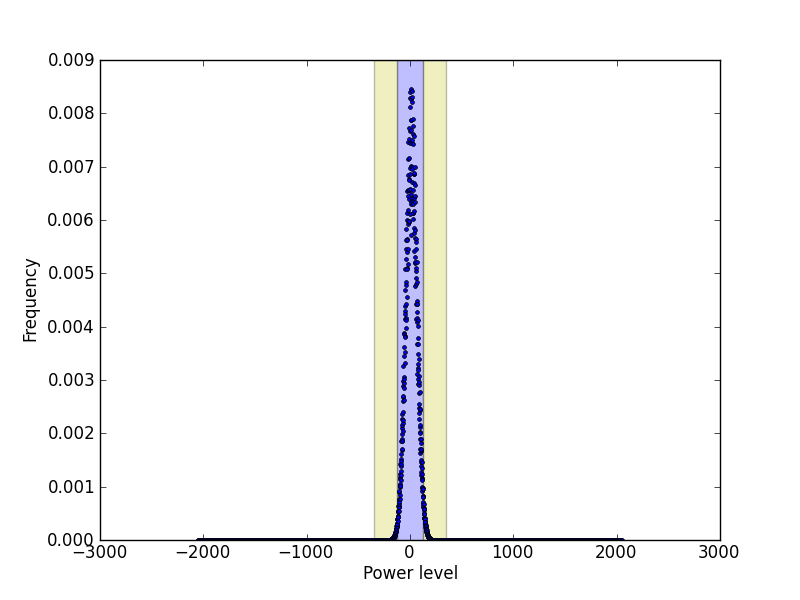
\includegraphics[width=0.5\textwidth]{plots/Stand010Xhist.png}} 				\subfloat{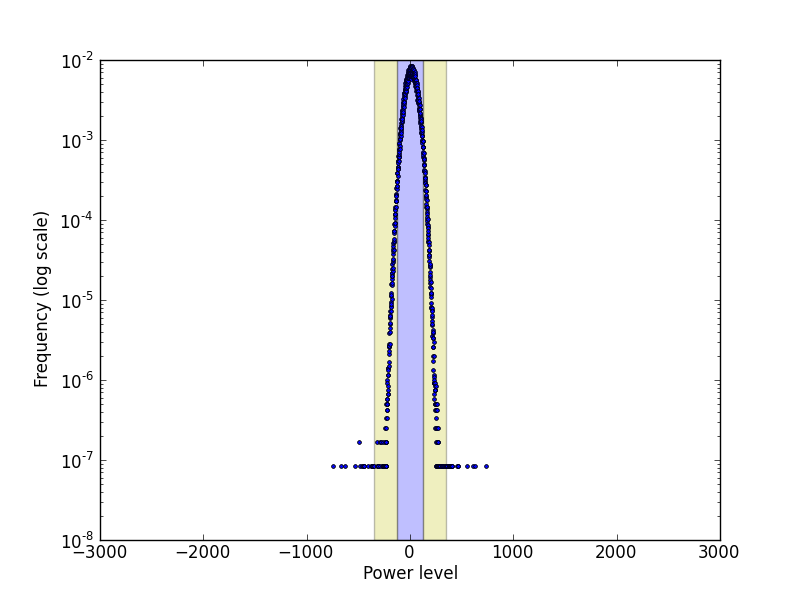
\includegraphics[width=0.5\textwidth]{plots/Stand010Xhist_log.png}} 				\caption{Data from Stand010X. RMS is 55.1743 Samples used : 3792000000. If the RMS is unchanged 98.0064 percent of the samples will lie within [-128,128).  				 With an RMS of 20, 99.9997 percent of the samples will lie within [-128,128).} 				\end{figure} 

\begin{figure}[h] 				\subfloat{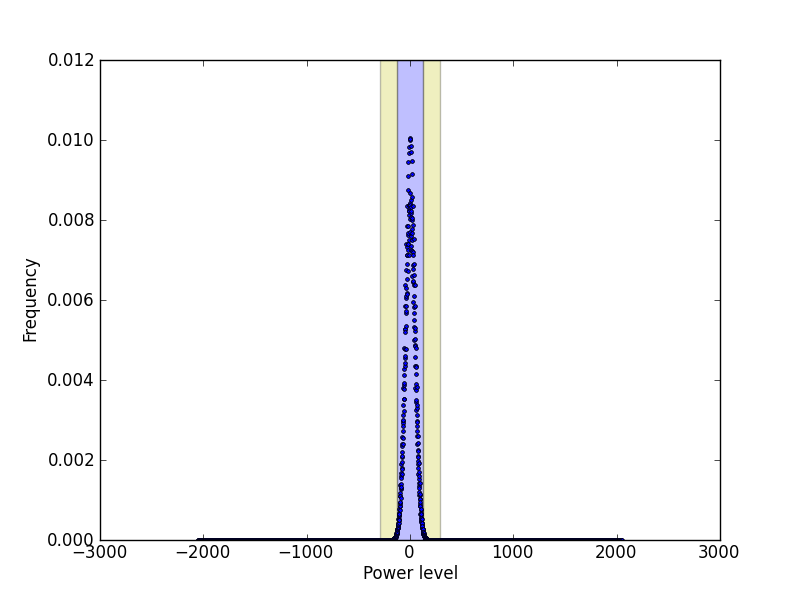
\includegraphics[width=0.5\textwidth]{plots/Stand010Yhist.png}} 				\subfloat{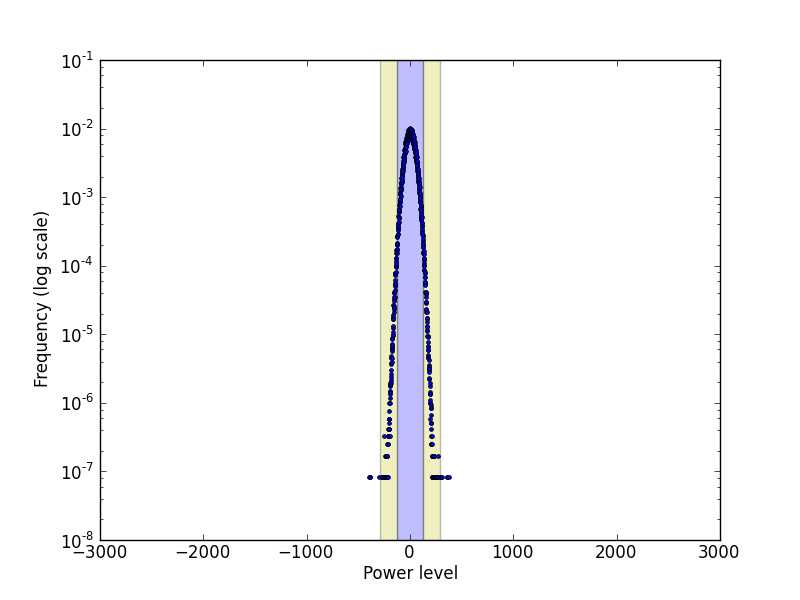
\includegraphics[width=0.5\textwidth]{plots/Stand010Yhist_log.png}} 				\caption{Data from Stand010Y. RMS is 46.1129 Samples used : 3792000000. If the RMS is unchanged 99.4528 percent of the samples will lie within [-128,128).  				 With an RMS of 20, 99.9999 percent of the samples will lie within [-128,128).} 				\end{figure} 

\begin{figure}[h] 				\subfloat{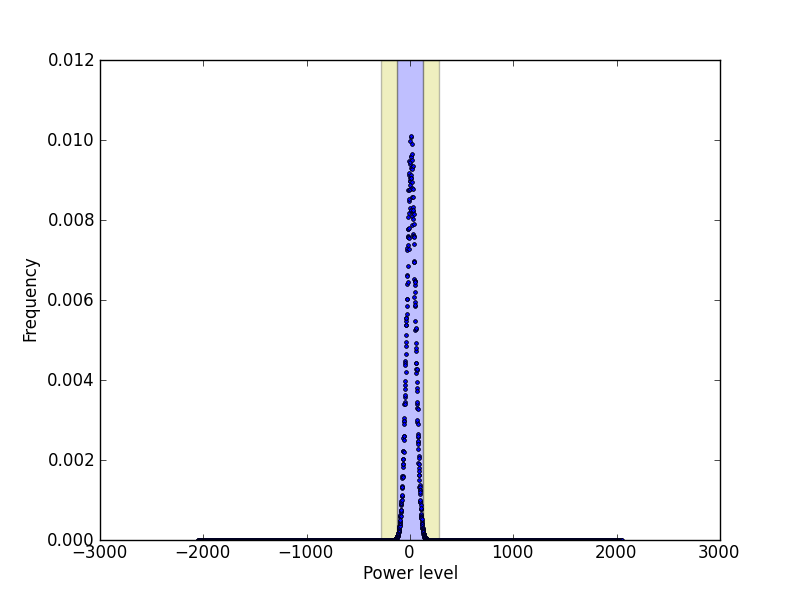
\includegraphics[width=0.5\textwidth]{plots/Stand054Xhist.png}} 				\subfloat{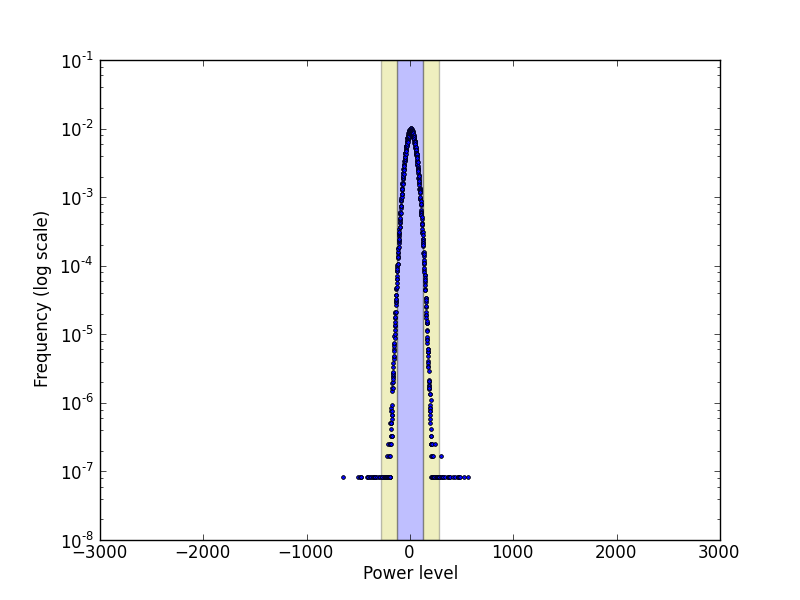
\includegraphics[width=0.5\textwidth]{plots/Stand054Xhist_log.png}} 				\caption{Data from Stand054X. RMS is 43.7177 Samples used : 3792000000. If the RMS is unchanged 99.6627 percent of the samples will lie within [-128,128).  				 With an RMS of 20, 99.9996 percent of the samples will lie within [-128,128).} 				\end{figure} 

\begin{figure}[h] 				\subfloat{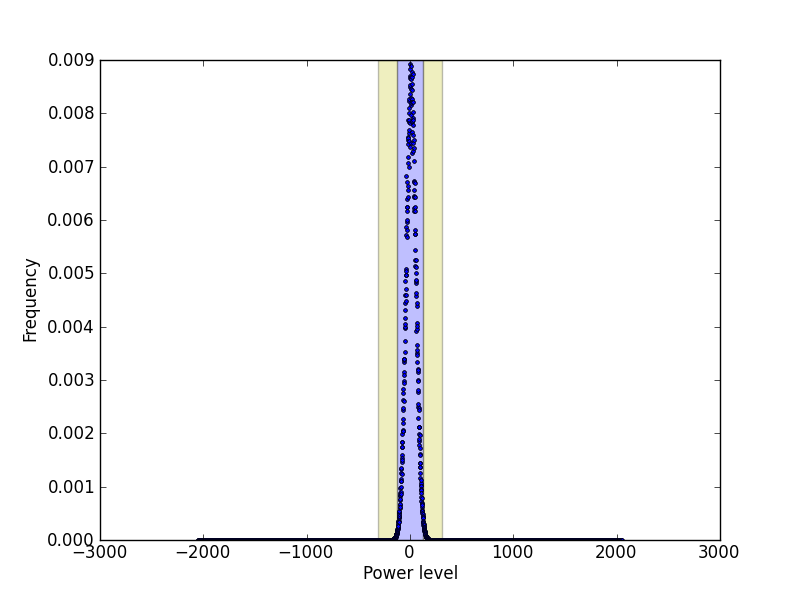
\includegraphics[width=0.5\textwidth]{plots/Stand054Yhist.png}} 				\subfloat{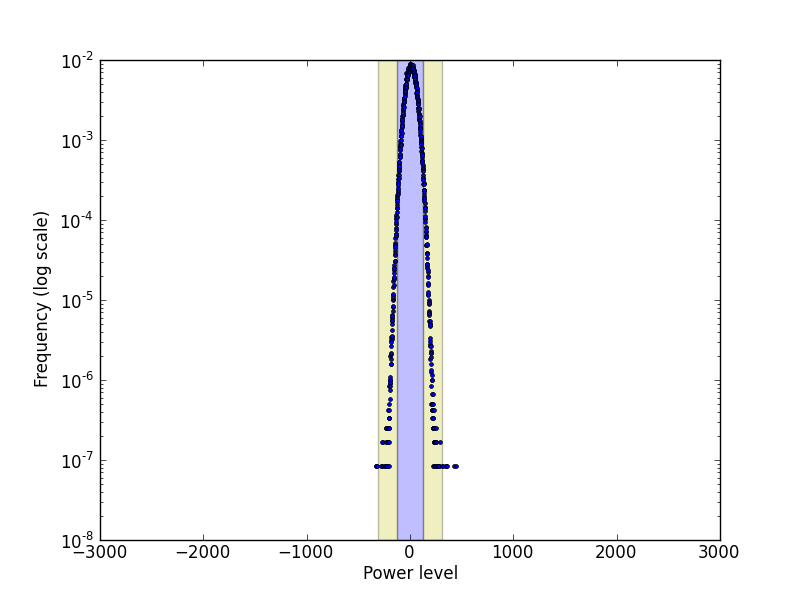
\includegraphics[width=0.5\textwidth]{plots/Stand054Yhist_log.png}} 				\caption{Data from Stand054Y. RMS is 47.8891 Samples used : 3792000000. If the RMS is unchanged 99.2436 percent of the samples will lie within [-128,128).  				 With an RMS of 20, 99.9999 percent of the samples will lie within [-128,128).} 				\end{figure} 

\begin{figure}[h] 				\subfloat{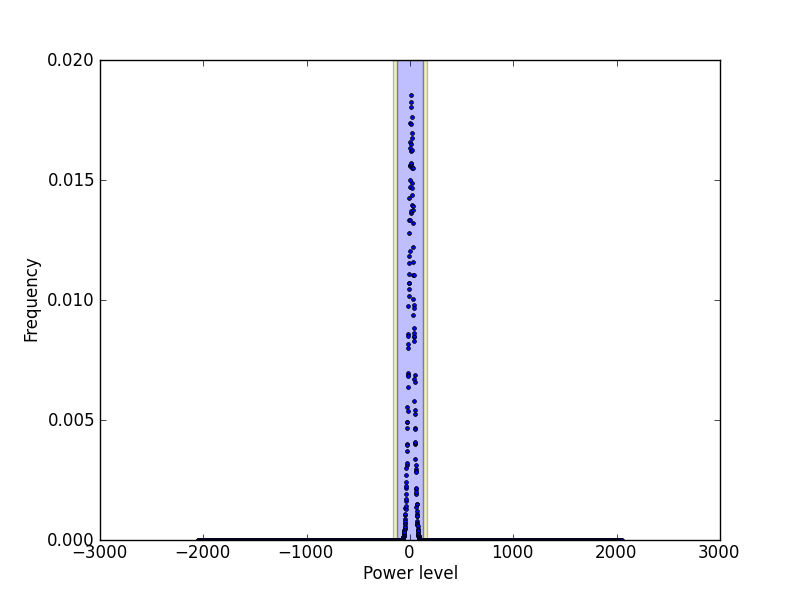
\includegraphics[width=0.5\textwidth]{plots/Stand248Xhist.png}} 				\subfloat{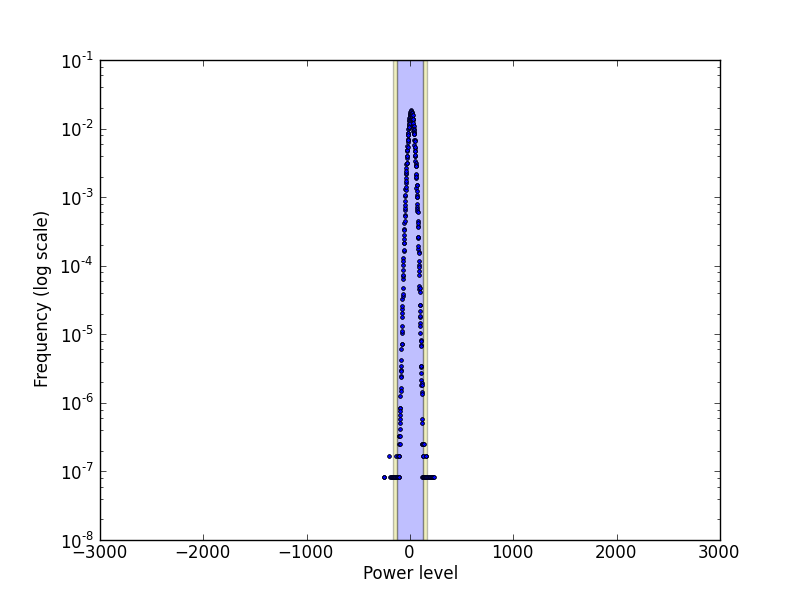
\includegraphics[width=0.5\textwidth]{plots/Stand248Xhist_log.png}} 				\caption{Data from Stand248X. RMS is 26.1238 Samples used : 3792000000. If the RMS is unchanged 99.9996 percent of the samples will lie within [-128,128).  				 With an RMS of 20, 99.9998 percent of the samples will lie within [-128,128).} 				\end{figure} 

\begin{figure}[h] 				\subfloat{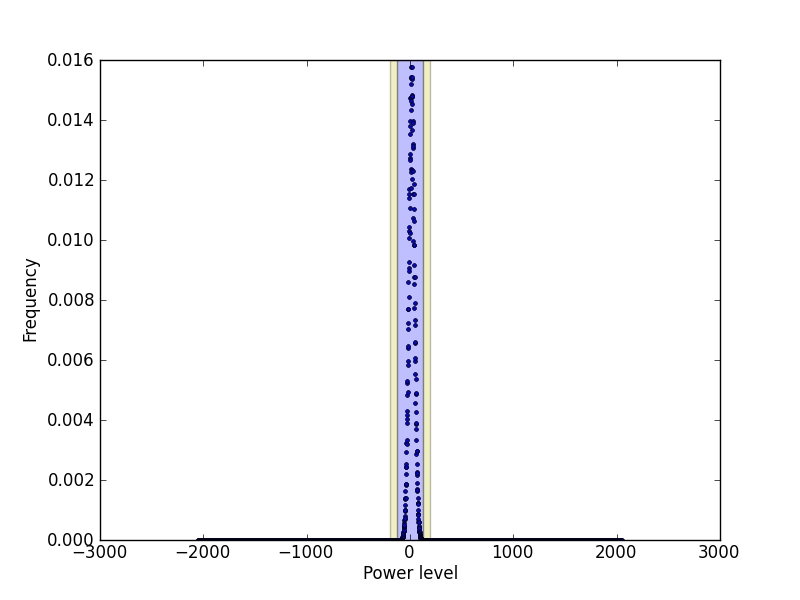
\includegraphics[width=0.5\textwidth]{plots/Stand248Yhist.png}} 				\subfloat{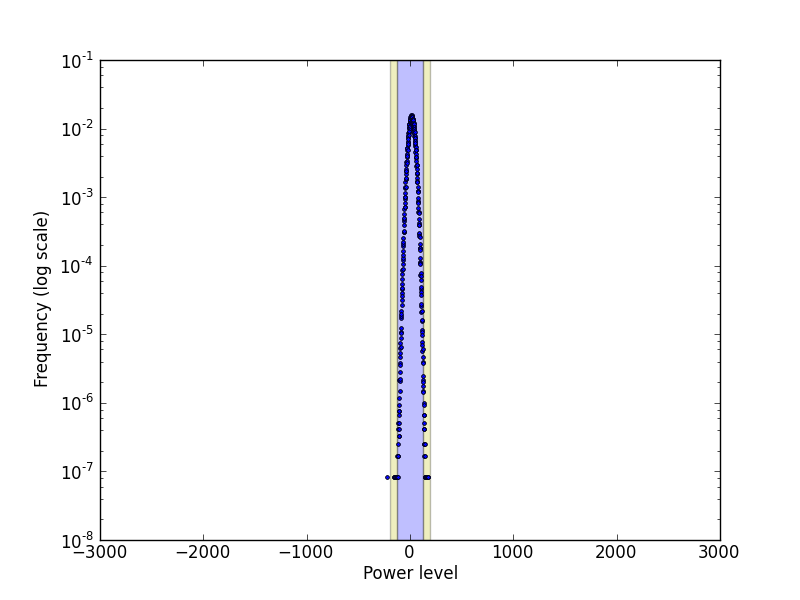
\includegraphics[width=0.5\textwidth]{plots/Stand248Yhist_log.png}} 				\caption{Data from Stand248Y. RMS is 30.7076 Samples used : 3792000000. If the RMS is unchanged 99.9988 percent of the samples will lie within [-128,128).  				 With an RMS of 20, 100.0000 percent of the samples will lie within [-128,128).} 				\end{figure} 

\begin{figure}[h] 				\subfloat{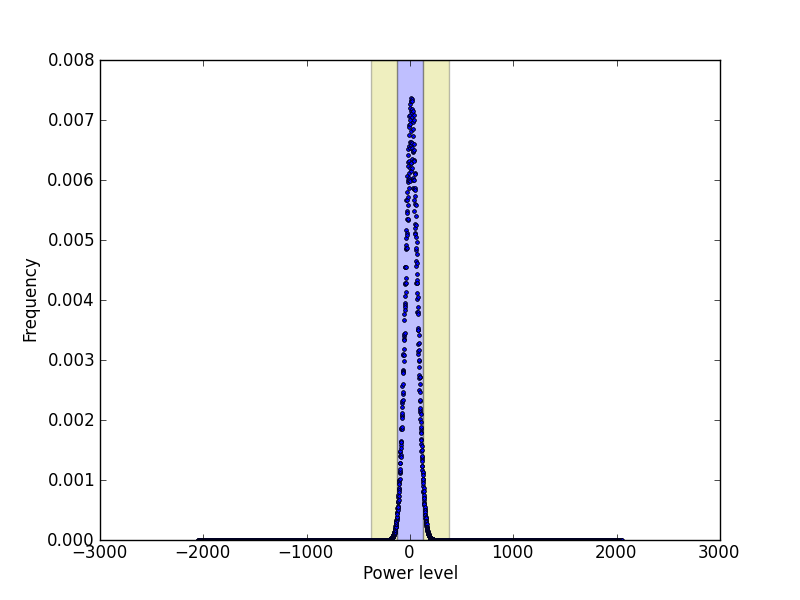
\includegraphics[width=0.5\textwidth]{plots/Stand251Xhist.png}} 				\subfloat{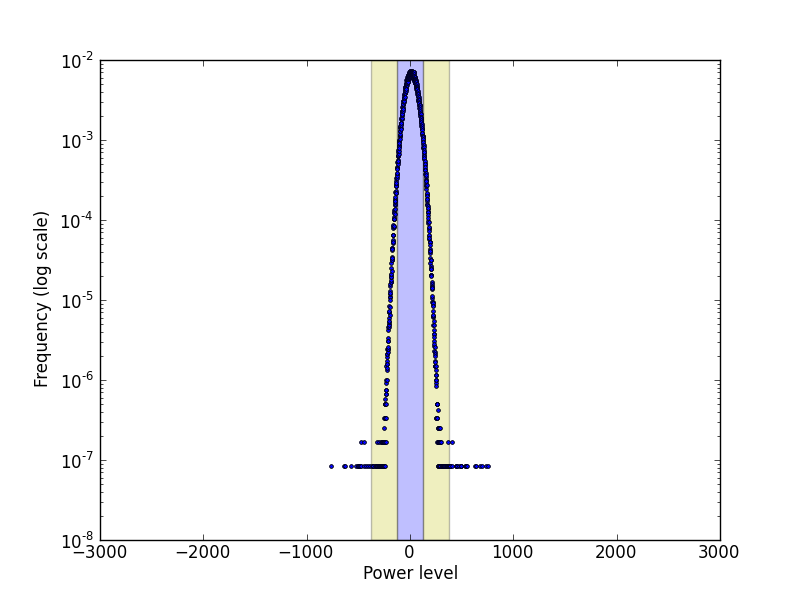
\includegraphics[width=0.5\textwidth]{plots/Stand251Xhist_log.png}} 				\caption{Data from Stand251X. RMS is 58.7564 Samples used : 3792000000. If the RMS is unchanged 97.0939 percent of the samples will lie within [-128,128).  				 With an RMS of 20, 99.9996 percent of the samples will lie within [-128,128).} 				\end{figure} 

\begin{figure}[h] 				\subfloat{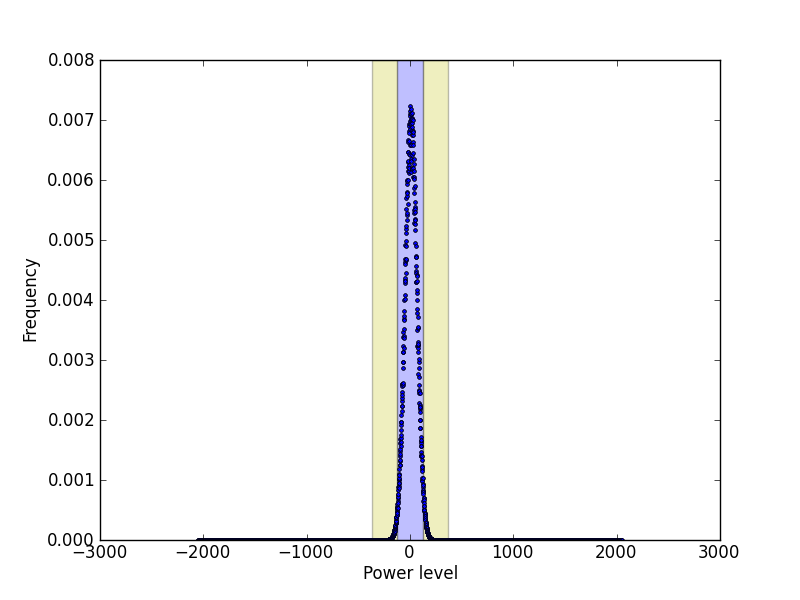
\includegraphics[width=0.5\textwidth]{plots/Stand251Yhist.png}} 				\subfloat{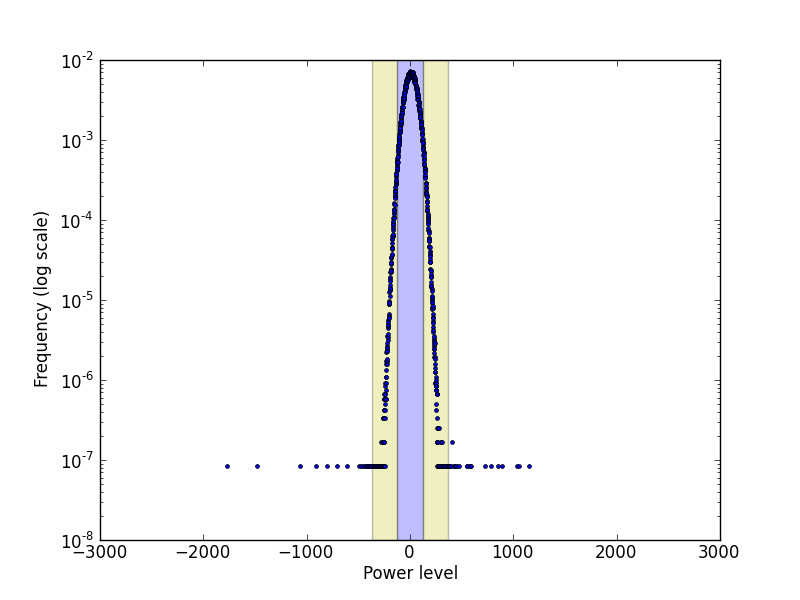
\includegraphics[width=0.5\textwidth]{plots/Stand251Yhist_log.png}} 				\caption{Data from Stand251Y. RMS is 58.0470 Samples used : 3792000000. If the RMS is unchanged 97.2851 percent of the samples will lie within [-128,128).  				 With an RMS of 20, 99.9997 percent of the samples will lie within [-128,128).} 				\end{figure} 

\begin{figure}[h] 				\subfloat{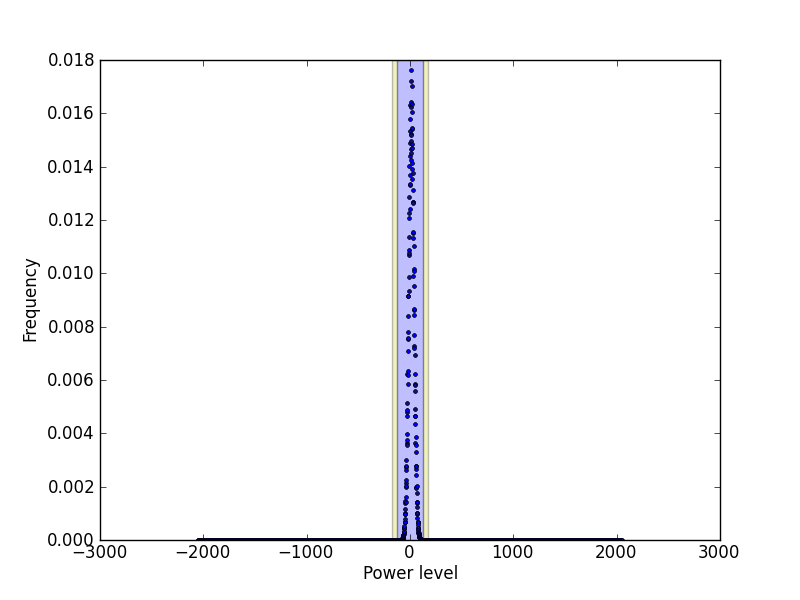
\includegraphics[width=0.5\textwidth]{plots/Stand258Xhist.png}} 				\subfloat{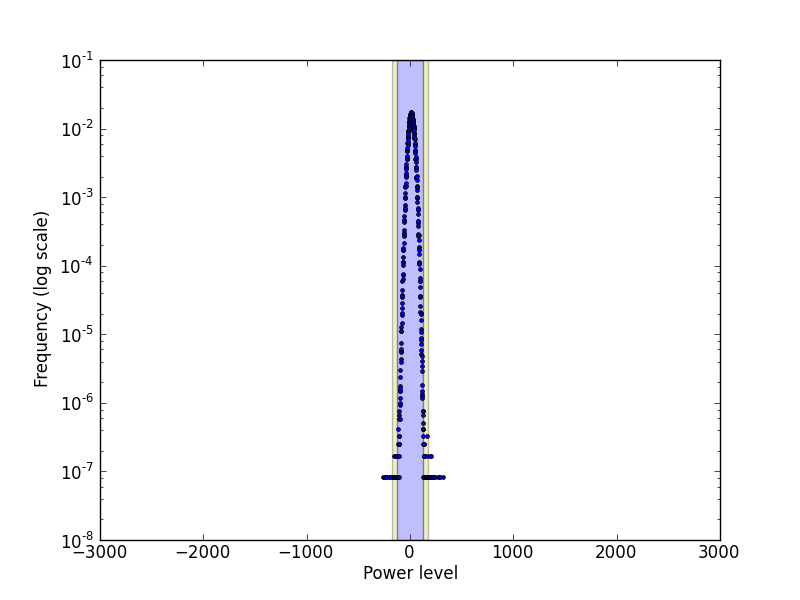
\includegraphics[width=0.5\textwidth]{plots/Stand258Xhist_log.png}} 				\caption{Data from Stand258X. RMS is 27.4041 Samples used : 3792000000. If the RMS is unchanged 99.9993 percent of the samples will lie within [-128,128).  				 With an RMS of 20, 99.9998 percent of the samples will lie within [-128,128).} 				\end{figure} 

\begin{figure}[h] 				\subfloat{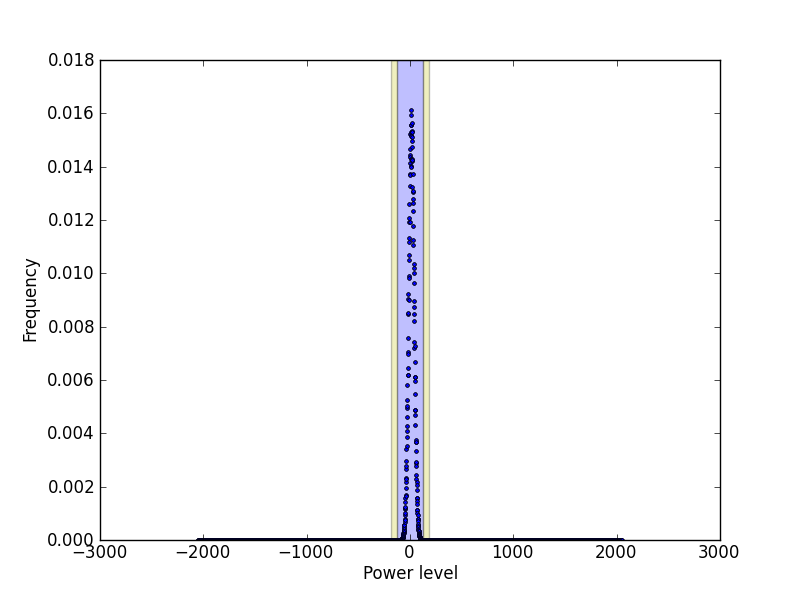
\includegraphics[width=0.5\textwidth]{plots/Stand258Yhist.png}} 				\subfloat{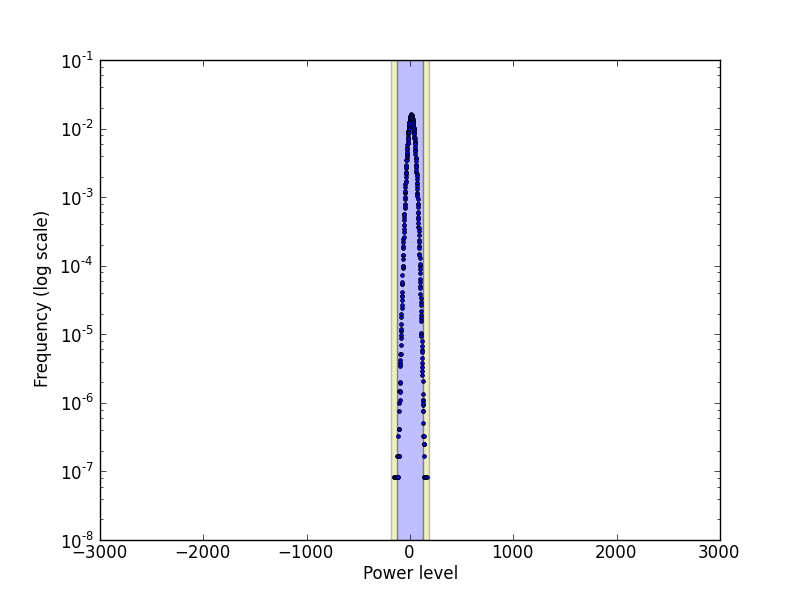
\includegraphics[width=0.5\textwidth]{plots/Stand258Yhist_log.png}} 				\caption{Data from Stand258Y. RMS is 28.3805 Samples used : 3792000000. If the RMS is unchanged 99.9995 percent of the samples will lie within [-128,128).  				 With an RMS of 20, 100.0000 percent of the samples will lie within [-128,128).} 				\end{figure} 



\end{document}